\documentclass[11pt]{article}
\usepackage[utf8]{inputenc}
\usepackage{fontspec}
\usepackage{amsmath}
\usepackage{amssymb}
\usepackage{hyperref}
\usepackage[margin=1.2in]{geometry}
\usepackage{booktabs}
\usepackage{enumitem}
\usepackage{parskip}
\usepackage{setspace}
\usepackage{graphicx}
\usepackage[table]{xcolor}
\usepackage{pagecolor}
\usepackage{listings}

% Style rules
\setstretch{1.15}
\setcounter{secnumdepth}{0}
\date{}

% Dark mode styling
\definecolor{darkbg}{HTML}{1E1E1E}
\definecolor{lighttext}{HTML}{D4D4D4}
\pagecolor{darkbg}
\color{lighttext}

\hypersetup{
    colorlinks=true,
    linkcolor=cyan,
    citecolor=cyan,
    filecolor=cyan,
    urlcolor=cyan
}

% Code block styling
\lstset{
    backgroundcolor=\color{darkbg},
    basicstyle=\color{lighttext}\ttfamily\small,
    breaklines=true,
    frame=single,
    rulecolor=\color{lighttext},
    commentstyle=\color{gray},
    keywordstyle=\color{cyan},
    stringstyle=\color{orange}
}

\title{STOP Using AdamW, EVERYONE Uses Muon Now}
\author{Vuk Rosić, reviewed by Chaoqi Liang \\ \small \raisebox{-0.2\height}{
\includegraphics[width=0.02\textwidth]{/Users/vukrosic/AI Science Projects/muon-course/.agent/skills/md-to-pdf/github.jpg}} \texttt{vukrosic/muon-optimizer-guide}}

\begin{document}
\maketitle

Everyone (OpenAI, Meta, DeepSeek, Moonshot AI,...) replaced AdamW with Muon optimizer to train their LLMs and neural networks.

DeepSeek researcher said that Muon optimizer was one of 2 biggest inventions in 2025.

\textbf{PyTorch 2.10 has official implementation of Muon!!!}


If you train ANY neural network - you MUST try it!

It should make your training 30\% to 2x faster!

\subsection{Evidence that Muon beats AdamW}

\begin{center}
    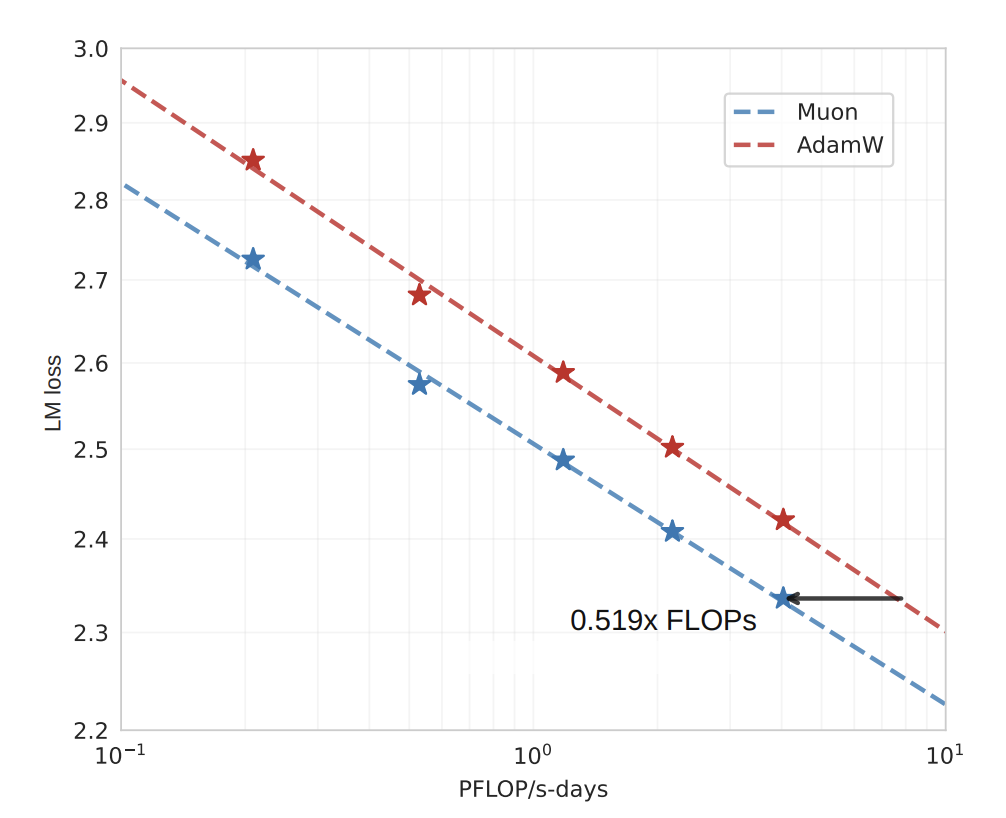
\includegraphics[width=0.8\textwidth]{images/muon_vs_adamw_kimi.png}
    
    Figure 1: \textit{Muon is effective on large-scale LLMs.} \href{https://arxiv.org/abs/2502.16982}{[MUON IS SCALABLE FOR LLM TRAINING on arxiv]}
\end{center}

Different optimizers to same loss as fast as possible, with as few tokens as possible:

\begin{center}
    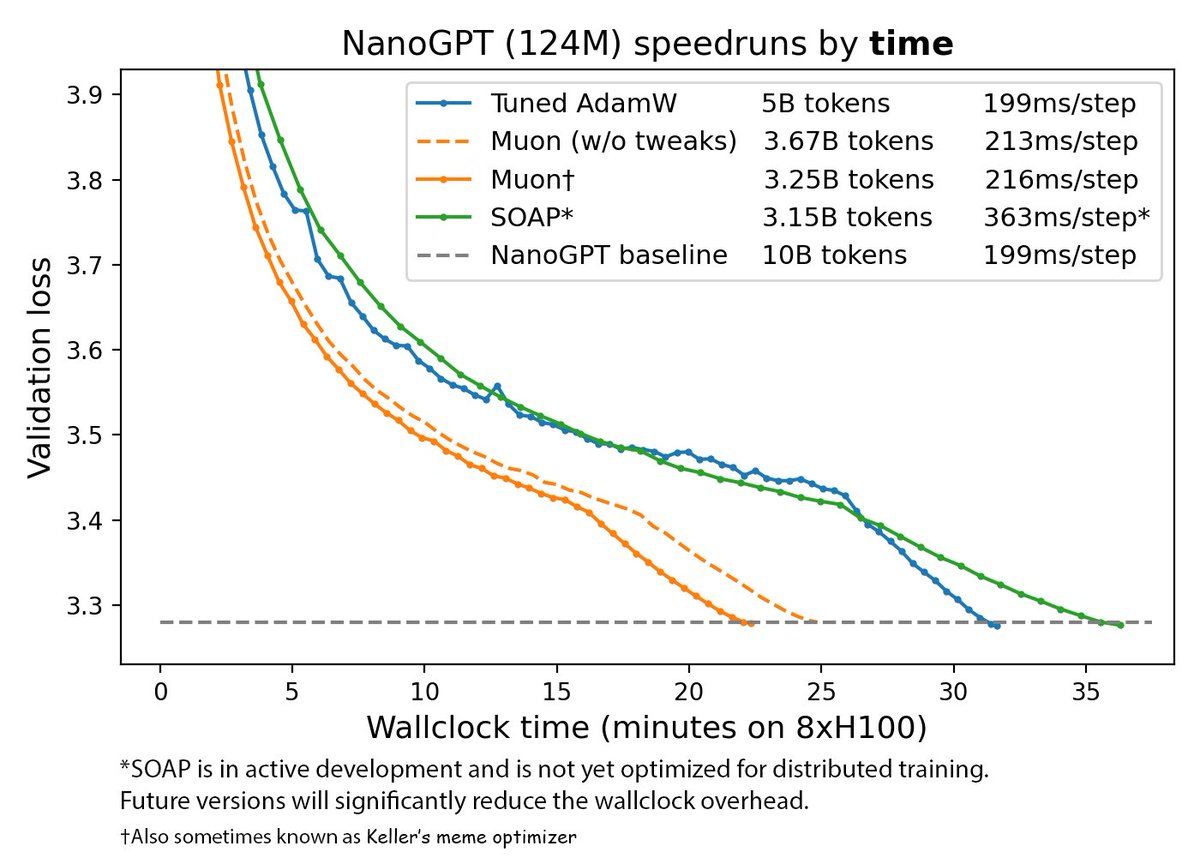
\includegraphics[width=0.8\textwidth]{images/nanogpt_curves.jpg}
    
    Figure 2: \textit{Faster LLM training.} \href{https://kellerjordan.github.io/posts/muon/}{[Jordan et al. 2024]}
\end{center}

\begin{quote}
    For code \& implementation scroll below.
\end{quote}

\section{The main idea}

If you are a beginner and don't understand any of this, please copy it into Gemini, ChatGPT, Claude, Kimi, etc. and ask it to teach you.

Let's start with the basic formula for weight updates:

\[
\theta_{t+1} = \theta_t - \eta \cdot \nabla_{\theta} \mathcal{L}
\]

\begin{itemize}
    \item $\theta_t$: Model parameters (all weights) at step $t$.
    \item $\theta_{t+1}$: Updated parameters after one training step.
    \item $\eta$: Learning rate (update step size).
    \item $\mathcal{L}$: Loss function.
    \item $\nabla_{\theta} \mathcal{L}$: Gradient of the loss with respect to parameters $\theta$.
    \item $t$: Optimization step index.
\end{itemize}

If we take a look at the gradients $\nabla_{\theta} \mathcal{L}$, this matrix is subtracted from weights - this is how neural network learns, however, this matrix might be ill-conditioned - some directions might have a strong ``pull'', while other directions might have a weak ``pull''.

\begin{center}
    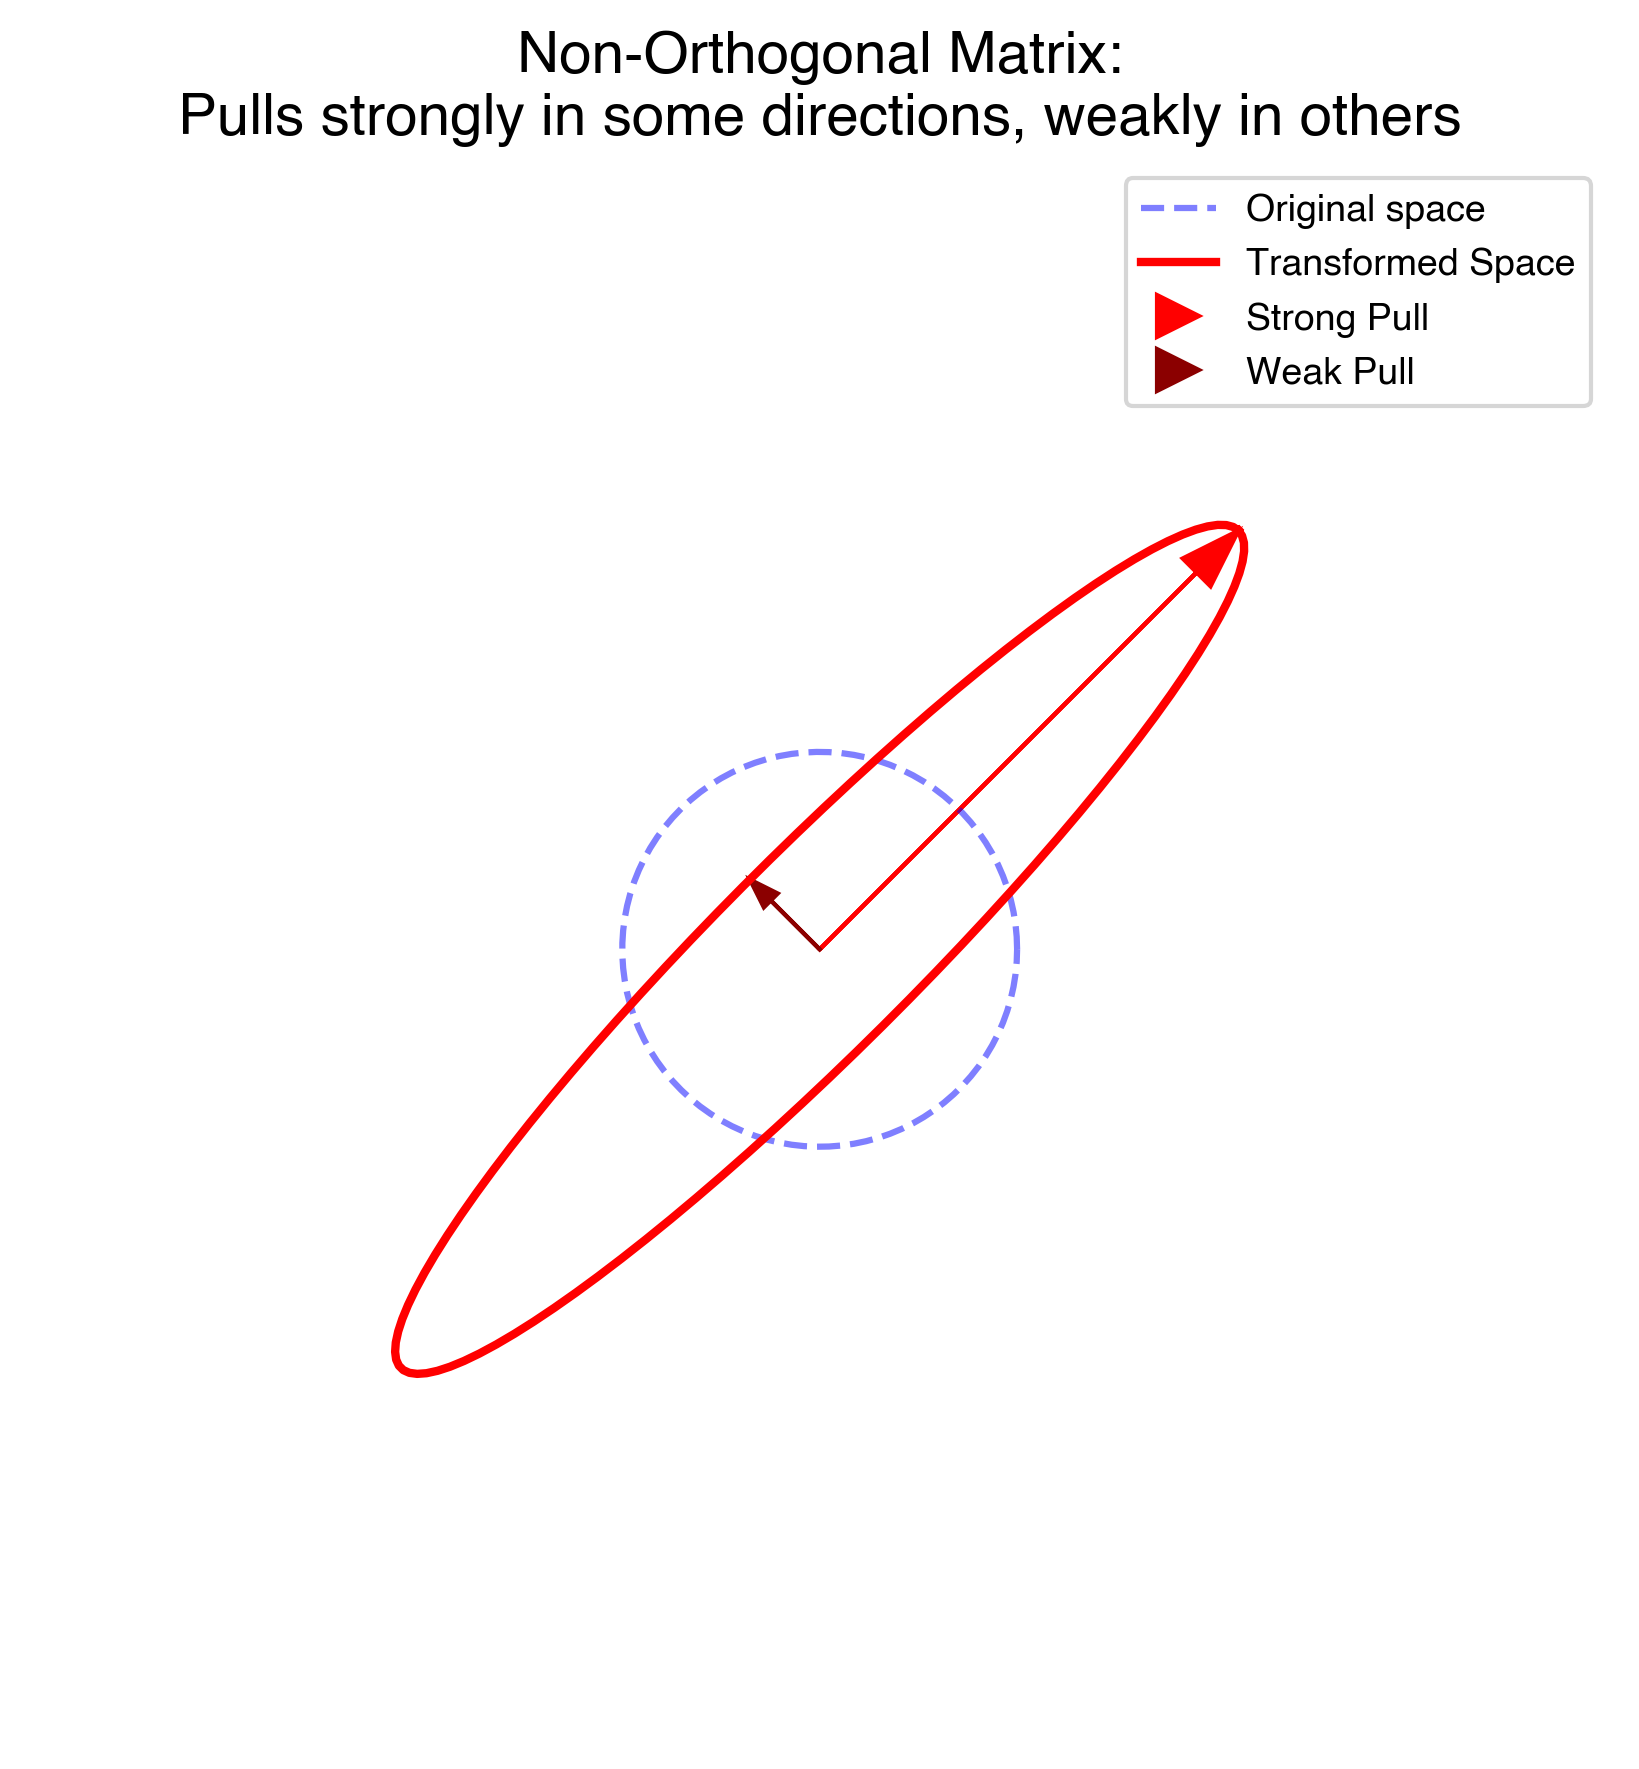
\includegraphics[width=0.8\textwidth]{images/01_non_orthogonal_effect.png}
    
    Non-Orthogonal Effects
\end{center}

A ``direction'' or a ``pull'' is a coordinated change across multiple weights. It controls an input$\to$output pathway through a layer.

Example:
Let's say we are training a neural network - when it sees a lot of green color it should predict ``grass'', and when it sees a lot of circles, it should predict ``wheels''.

Due to different types of encoding images, it might turn out that green image gradients have very small singular values (0.01), while circle image gradients have larger singular values (100).

This means that neural network will learn the [green $\to$ grass] pathway (prediction) A LOT SLOWER than the [circle $\to$ wheels] pathway.

It's not that there is less data for green color or circles are more important, it's just about the way data is represented with numbers.

Muon optimizer solves this:

\begin{center}
    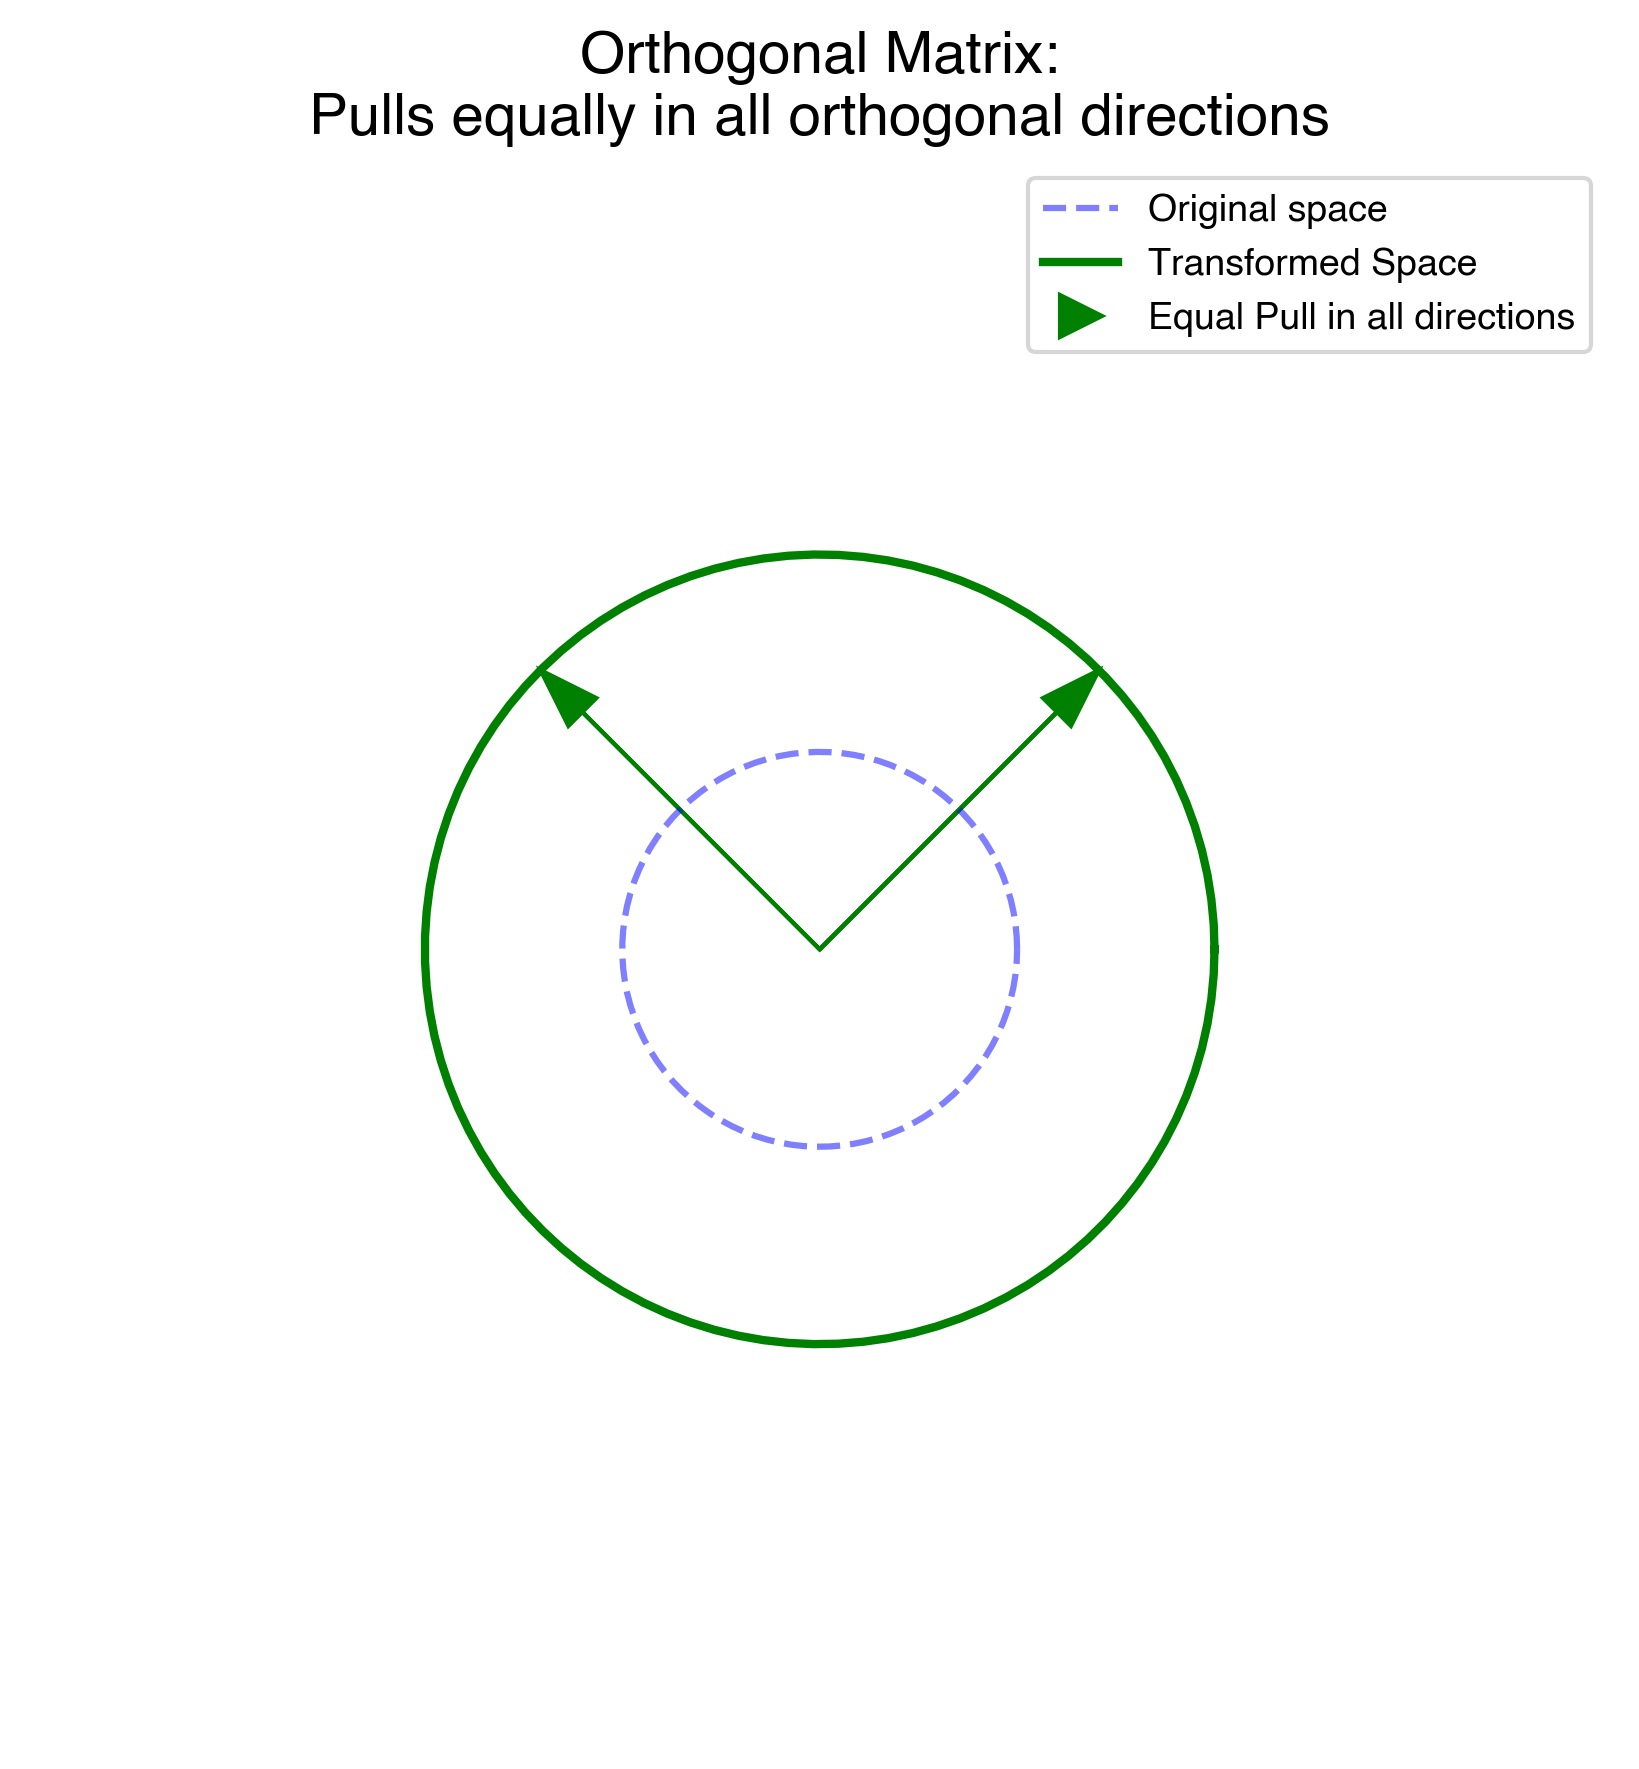
\includegraphics[width=0.8\textwidth]{images/01_orthogonal_effect.png}
    
    Orthogonal Effects
\end{center}

\begin{center}
    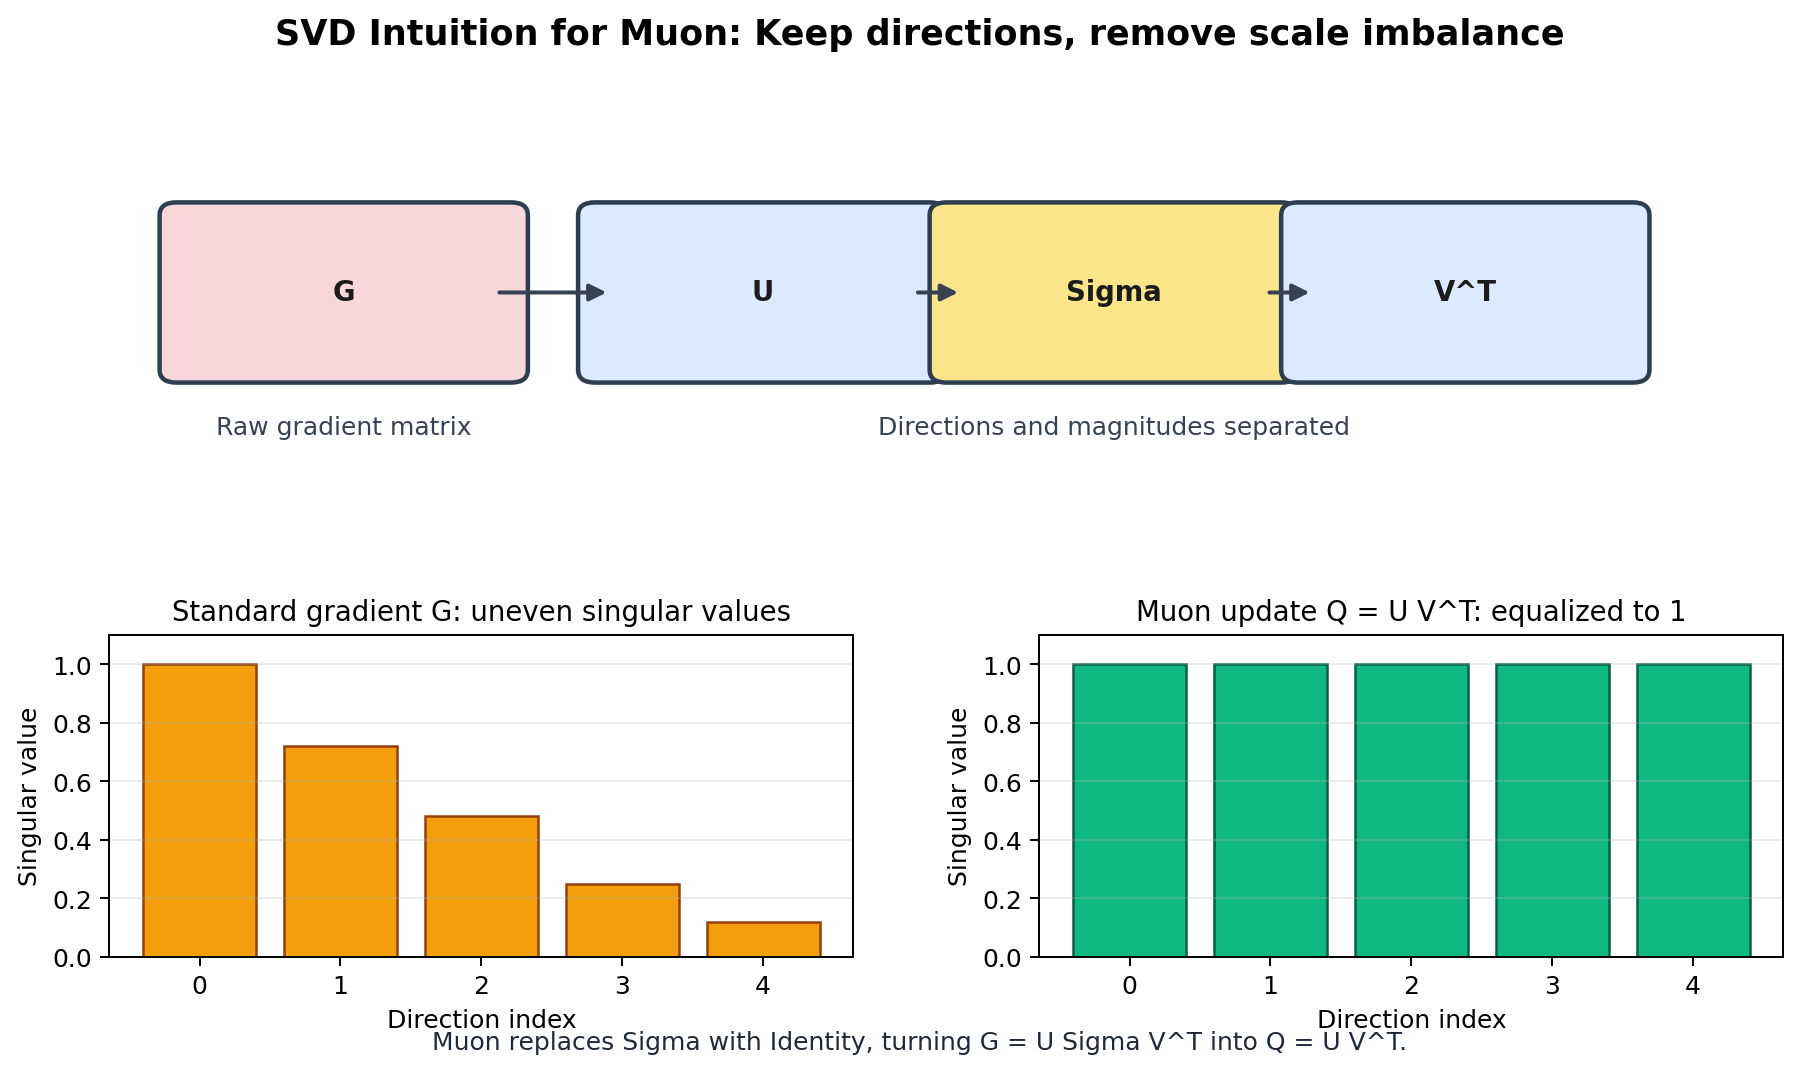
\includegraphics[width=0.8\textwidth]{images/03a_svd_for_muon_intro.png}
    
    SVD intuition for Muon: raw gradient has uneven singular values, while Muon uses UV\textsuperscript{T} with equalized singular values.
\end{center}

Muon optimizer will make all singular values equal to 1 (actually near 1, for faster computation), so it will update / learn [green $\to$ grass] pathway at the same speed as [circle $\to$ wheels] pathway.

\textbf{IMPORTANT}: Use Muon only for 2D weight matrices. Do NOT use it for embeddings, biases, LayerNorms, or the final output head - use AdamW for those.

\subsubsection{Crucial distinction}

Muon optimizer makes \textbf{weight update matrices} orthogonal, not the weight matrices.

\section{Code \& Implementation}

\textbf{UPDATE:} PyTorch 2.10 now includes an official implementation of Muon! You can find it under \texttt{torch.optim.Muon}.

\textbf{Performance Note:} My implementation below uses \href{https://arxiv.org/abs/2505.16932}{Polar Express} and typically works faster. However, if you prefer simplicity, you can use the official PyTorch implementation or the \href{https://github.com/KellerJordan/Muon/blob/master/muon.py}{original Keller Jordan code}.


If you copy paste the code into your AI agent, it should automatically implement it.

\begin{lstlisting}[language=Python]
import torch

# Polar Express coefficients - each step uses different, pre-optimized (a, b, c).
coeffs_list = [
    (8.156554524902461,  -22.48329292557795,   15.878769915207462),
    (4.042929935166739,  -2.808917465908714,    0.5000178451051316),
    (3.8916678022926607, -2.772484153217685,    0.5060648178503393),
    (3.285753657755655,  -2.3681294933425376,   0.46449024233003106),
    (2.3465413258596377, -1.7097828382687081,   0.42323551169305323),
]

@torch.compile()
def zeropower_polar_express(G: torch.Tensor, steps: int = 5) -> torch.Tensor:
    X = G.bfloat16()
    transposed = X.size(-2) > X.size(-1)
    if transposed:
        X = X.mT
    X = X / (X.norm(dim=(-2, -1), keepdim=True) * 1.01 + 1e-7)
    for a, b, c in coeffs_list[:steps]:
        A = X @ X.mT
        X = a * X + (b * A + c * A @ A) @ X
    return X.mT if transposed else X

class Muon(torch.optim.Optimizer):
    def __init__(self, params, lr: float = 0.02, momentum: float = 0.95,
                 weight_decay: float = 0.0):
        super().__init__(params, dict(lr=lr, momentum=momentum,
                                     weight_decay=weight_decay))

    @torch.no_grad()
    def step(self):
        for group in self.param_groups:
            for p in group["params"]:
                if p.grad is None:
                    continue
                state = self.state[p]
                if "buf" not in state:
                    state["buf"] = torch.zeros_like(p.grad)
                buf = state["buf"]
                buf.lerp_(p.grad, 1 - group["momentum"])
                g = p.grad.lerp_(buf, group["momentum"])
                g = zeropower_polar_express(g.view(g.size(0), -1))
                g = g.to(p.dtype)
                if group["weight_decay"] > 0:
                    p.mul_(1 - group["lr"] * group["weight_decay"])
                scale = max(1, p.size(-2) / p.size(-1)) ** 0.5
                p.add_(g.view_as(p), alpha=-group["lr"] * scale)
\end{lstlisting}

\begin{description}
    \item[Note:] For quick use, just copy-paste the code above. For more control, grab \texttt{optimizers/muon.py}.
\end{description}

\subsection{Usage Example}

\begin{lstlisting}[language=Python]
import torch
import torch.nn as nn

model = MyTransformer().cuda()

muon_params  = [p for p in model.parameters() if p.ndim == 2 and p.requires_grad]
adamw_params = [p for p in model.parameters() if not (p.ndim == 2 and p.requires_grad)]

optimizer_muon  = Muon(muon_params,  lr=0.02, momentum=0.95)
optimizer_adamw = torch.optim.AdamW(adamw_params, lr=3e-4, weight_decay=0.1)

for batch in dataloader:
    loss = model(batch)
    loss.backward()
    optimizer_muon.step()
    optimizer_adamw.step()
    optimizer_muon.zero_grad()
    optimizer_adamw.zero_grad()
\end{lstlisting}

\begin{description}
    \item[Tip:] A simple \texttt{p.ndim == 2} filter correctly separates Linear weight matrices.
\end{description}

\subsection{Key Implementation Tips}

\subsubsection{Use a BIG Learning Rate}
Unlike AdamW which typically uses \texttt{3e-4}, Muon works best with much larger learning rates:
\begin{itemize}
    \item \textbf{Default:} \texttt{0.02}.
    \item \textbf{Range:} \texttt{0.01} to \texttt{0.05}.
\end{itemize}

\subsubsection{Parameter Routing}
Muon is designed for 2-D weight matrices only. Use AdamW for everything else.

\subsubsection{Compile It!}
Use \texttt{@torch.compile()} for performance.

\subsubsection{Scaling the LR by Matrix Shape}
The update is scaled by $\sqrt{\max(1, \text{rows} / \text{cols})}$.

\end{document}
